\documentclass{article}
\usepackage[utf8]{inputenc}
\usepackage{hyperref}
\usepackage{amsmath,amssymb}
\usepackage{graphicx}
\usepackage{float}
\usepackage{booktabs}
\usepackage[margin=2.5cm]{geometry}
\usepackage[
  backend=biber,
  style=alphabetic,
]{biblatex}

\newcommand{\mbf}[1]{\mathbf{#1}}
\newcommand{\be}{\begin{equation}}
\newcommand{\ee}{\end{equation}}
\newcommand{\mcl}[1]{\mathcal{#1}}
\newcommand{\bsigma}{\boldsymbol{\sigma}}
\newcommand{\beps}{\boldsymbol{\varepsilon}}


\title{Cloaking experiments with Nassar-type metamaterials\vspace{-1em}}
\addbibresource{sample.bib}
\author{(notes)}
\date{}

\begin{document}
\maketitle
\tableofcontents

%% ==================================================================
\section{Simple homogenization schema of Nassar-type unit cells}
%% ==================================================================

\subsection{Transformation elasticity and the BGM gauge}

An elastic cloak is an annular coating $\{r_i < \|\mbf{x}\| < r_c\}$ that
renders a void $\{\|\mbf{x}\| < r_i\}$ invisible to elastic waves.
The constitutive properties of the coating follow from a
blow-up coordinate transformation $\mbf{x} = \boldsymbol{\phi}(\mbf{X})$
that maps the origin to the circle of radius~$r_i$~\cite{brun2009}.

Under the Brun--Guenneau--Movchan (BGM) gauge, the transformed
elasticity tensor and mass density are~\cite{nassar2018}
\be\label{eq:pushforward}
  c_{ijkl}
  = \frac{F_{jm}\,F_{ln}\,C_{imkn}}{J}\,,
  \qquad
  \rho = \frac{R}{J}\,,
\ee
where $\mbf{F} = \partial\mbf{x}/\partial\mbf{X}$ is the deformation
gradient, $J = \det\mbf{F}$, $\mbf{C}$ and~$R$ are the background
stiffness and density.
The transformed tensor~$\mbf{c}$ breaks the minor symmetries
($c_{ijkl} \neq c_{jikl}$) while preserving major symmetry
($c_{ijkl} = c_{klij}$).
A material realising such a tensor is necessarily \emph{polar}
(it resists rotations via body torques) and \emph{degenerate}
(it admits a stressless collapse mechanism)~\cite{nassar2018}.

For the circular blow-up with an isotropic background
$(\lambda,\mu)$, the effective stiffness in the local polar
basis $(\mbf{m}, \mbf{n})$ = (radial, tangential) reads
\be\label{eq:Ceff}
  \mbf{c}_{\mathrm{eff}}
  =
  \begin{bmatrix}
    (2\mu{+}\lambda)\,f & \lambda & 0 & 0 \\
    \lambda & (2\mu{+}\lambda)/f & 0 & 0 \\
    0 & 0 & \mu/f & \mu \\
    0 & 0 & \mu & \mu f
  \end{bmatrix},
  \qquad
  f = \frac{\|\mbf{x}\| - r_i}{\|\mbf{x}\|}\,,
\ee
in augmented Voigt ordering
$[\sigma_{11},\sigma_{22},\sigma_{12},\sigma_{21}]$.
The effective density is position-dependent:
\be\label{eq:rhoeff}
  \rho_{\mathrm{eff}}
  = \frac{r_c^2}{(r_c - r_i)^2}\,f\,R\,.
\ee
Near the inner boundary ($r\to r_i$, $f\to 0$) the radial stiffness
and density vanish while the tangential stiffness diverges ---
perfect cloaking requires this singular behaviour, which can only be
approximated by a finite lattice.

% \subsection{The Nassar degenerate polar lattice}

% Nassar et al.~\cite{nassar2018} propose a lattice whose unit cell
% contains a rigid rectangular mass with two diagonal springs of
% constant~$\alpha$, one vertical spring of constant~$\beta$, and a
% torsion spring of constant~$\kappa$.
% The lattice is rectangular with cell dimensions $a$ (radial) and
% $b$ (tangential), tilted at angle~$\theta$ to the radial direction
% (Fig.~\ref{fig:polar_lattice}).

% The lattice's effective Hooke's law in augmented Voigt is
% \be\label{eq:nassar_forward}
%   \mbf{c}_{\mathrm{lat}}
%   =
%   \begin{bmatrix}
%     r\,c^2\alpha & cs\alpha & 0 & 0 \\
%     cs\alpha & (\alpha s^2{+}2\beta)/r & 0 & 0 \\
%     0 & 0 & c^2\alpha\kappa/\Delta & r\,cs\alpha\kappa/\Delta \\
%     0 & 0 & r\,cs\alpha\kappa/\Delta & r^2 s^2\alpha\kappa/\Delta
%   \end{bmatrix},
% \ee
% where $c = \cos\theta$, $s = \sin\theta$, $r = a/b$ is the cell
% aspect ratio, and $\Delta = \alpha(c-rs)^2 + r\kappa$.

% \subsection{Parameter identification}

% Matching~\eqref{eq:nassar_forward} to~\eqref{eq:Ceff} yields the
% design parameters that make the lattice reproduce the transformation
% cloaking tensor exactly.
% The global parameters (position-independent) are
% \be\label{eq:global_params}
%   \theta = \arctan\!\sqrt{\frac{\lambda}{2\mu+\lambda}}\,,
%   \quad
%   \alpha = 2(\mu+\lambda)\sqrt{\frac{\lambda}{2\mu+\lambda}}\,,
%   \quad
%   \beta = \frac{(2\mu+\lambda)^2 - \lambda^2}
%                {2\sqrt{\lambda}\,\sqrt{2\mu+\lambda}}\,,
% \ee
% and the position-dependent parameters (through $f$) are
% \be\label{eq:local_params}
%   \frac{a}{b} = f\,\sqrt{\frac{2\mu+\lambda}{\lambda}}\,,
%   \qquad
%   \kappa = \frac{\lambda\mu}{\lambda - \mu}
%            \,\frac{(1-f)^2}{f}\,.
% \ee
% Stability requires $\mu \leq \lambda$ so that $\kappa > 0$.
% In the special case $\lambda = \mu$, we obtain $\kappa\to\infty$
% (the lattice enforces minor symmetry) and $\theta = \pi/6$.

% \begin{figure}[H]
%   \centering
%   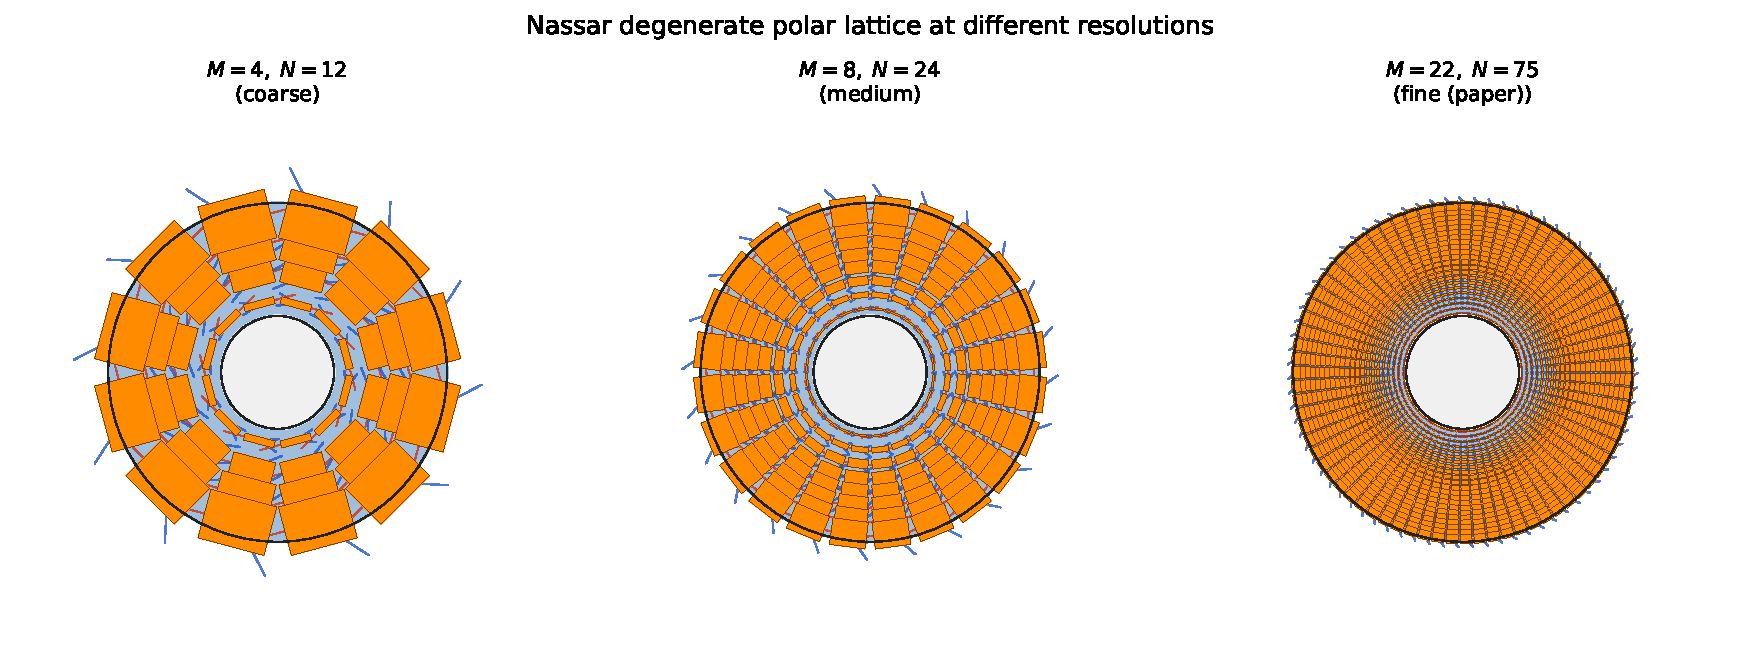
\includegraphics[width=\linewidth]{../figures/nassar_polar_lattice_resolutions.pdf}
%   \caption{Nassar degenerate polar lattice at three resolutions.
%   Each cell contains a rigid mass (orange), two diagonal springs~$\alpha$ (blue),
%   and one vertical spring~$\beta$ (red).
%   The innermost ring of cells cannot reach $r = r_i$ exactly;
%   cloaking becomes ideal only in the limit $M, N \to \infty$.}
%   \label{fig:polar_lattice}
% \end{figure}

\subsection{Homogenized cell model}

Instead of modelling the discrete lattice, we discretise the cloak
annulus into a regular Cartesian grid of $n_x \times n_y$ square cells
(Fig.~\ref{fig:cartesian_cells}).
Each cell whose centre lies in $\{r_i < r < r_c\}$ is assigned a
piecewise-constant effective stiffness $\mbf{c}_{\mathrm{lat}}$.
The density is set to~\eqref{eq:rhoeff}.
Cells outside the annulus retain the background material;
cells inside the void are removed from the mesh.

% Since the Nassar parameters are expressed in the local polar frame
% $(\mbf{m}, \mbf{n})$, the stiffness tensor must be rotated to the
% global Cartesian frame $(x, y)$ by the standard fourth-order rotation:
% \be
%   c_{ijkl}^{\mathrm{cart}}
%   = R_{ia}\,R_{jb}\,R_{kc}\,R_{ld}\;
%     c_{abcd}^{\mathrm{polar}}\,,
%   \qquad
%   \mbf{R}(\varphi)
%   = \begin{bmatrix}
%       \cos\varphi & -\sin\varphi \\
%       \sin\varphi & \phantom{-}\cos\varphi
%     \end{bmatrix},
% \ee
% where $\varphi = \mathrm{atan2}(y, x)$ is the polar angle of the cell
% centre.

\begin{figure}[H]
  \centering
  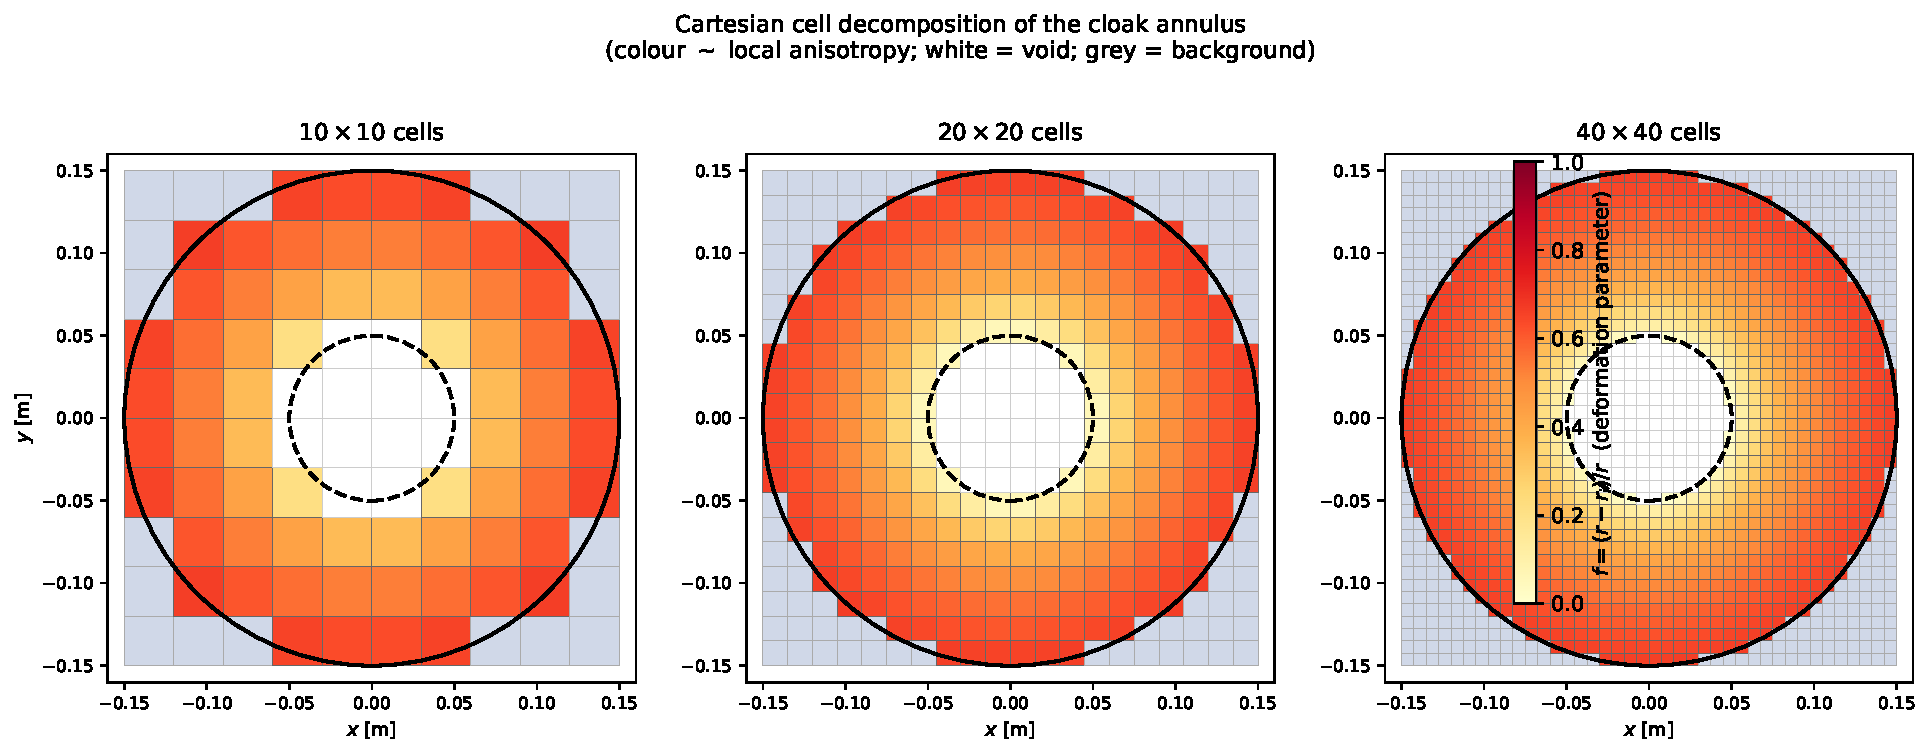
\includegraphics[width=\linewidth]{../figures/nassar_cartesian_cells.pdf}
  \caption{Cartesian cell decomposition of the cloak annulus at
  three grid resolutions.
  Colour encodes the deformation parameter
  $f = (r - r_i)/r$, which controls the local anisotropy;
  $f \to 0$ near $r_i$ (near-singular) and $f \to (r_c-r_i)/r_c$
  near $r_c$ (close to background).
  White cells lie inside the void; grey cells are background.
  Dashed/solid circles mark $r = r_i$ and $r = r_c$.}
  \label{fig:cartesian_cells}
\end{figure}


%% ==================================================================
\section{Circular cloaking of plane waves}
%% ==================================================================

\subsection{Simulation setup}

We consider a rectangular domain of side $4r_c = 0.6$\,m with
PML absorbing layers on all four boundaries.
A circular void of radius $r_i = 50$\,mm is centred in the domain,
coated by an annular cloak of outer radius $r_c = 150$\,mm.
The background medium is isotropic with
$\lambda = \mu = 2.5$\,MPa and $R = 2.7$\,kg/m$^2$ (plane stress).

The excitation is a Gaussian body-force line source at
$x = 0.15\,W$ from the left physical boundary, producing
approximately cylindrical pressure waves at $f = 40$\,kHz
(P-wave wavelength $\lambda_P \approx 42$\,mm, giving a void
diameter of $\approx 2.4\,\lambda_P$).
The frequency-domain elastodynamic equations are solved with
complex-valued DOFs and Rayleigh-damping PML via a JAX-FEM
finite-element solver on a triangular mesh with distance-based
refinement near the cloak boundaries
(${\sim}\,246{,}000$ elements, ${\sim}\,124{,}000$ nodes).

\subsection{Cloaking loss metric}

We define the cloaking distortion as the relative $L^2$ displacement
mismatch on the right physical boundary (the shadow side behind the
scatterer):
\be\label{eq:distortion}
  \mathcal{D}
  = 100\,\frac{\|\mbf{u}_{\mathrm{cloak}} - \mbf{u}_{\mathrm{ref}}\|_{L^2(\partial\Omega_{\mathrm{right}})}}
              {\|\mbf{u}_{\mathrm{ref}}\|_{L^2(\partial\Omega_{\mathrm{right}})}}\;\;[\%]\,,
\ee
where $\mbf{u}_{\mathrm{ref}}$ is the displacement in the intact
background (no void) and $\mbf{u}_{\mathrm{cloak}}$ is the solution
with void and cloak.
Perfect cloaking yields $\mathcal{D} = 0$.

\subsection{Results}

Three configurations are compared:
(i)~uncoated void (void present, no cloak),
(ii)~Nassar cell model at varying resolutions, and
(iii)~continuous $\mbf{c}_{\mathrm{eff}}$ from~\eqref{eq:Ceff}
(the theoretical optimum for the FEM discretisation).

\begin{table}[H]
\centering
\caption{Cloaking distortion $\mathcal{D}$ as a function of cell grid resolution.}
\label{tab:convergence}
\begin{tabular}{@{}lrr@{}}
\toprule
Configuration & Cloak cells & $\mathcal{D}$ [\%] \\
\midrule
Uncoated void     &    ---   & 70.31 \\
\midrule
Nassar $5\times5$     &    20  & 119.64 \\
Nassar $10\times10$   &    68  & 127.11 \\
Nassar $20\times20$   &   284  & 91.60 \\
Nassar $40\times40$   & 1\,124  & 73.74 \\
Nassar $60\times60$   & 2\,512  & 49.42 \\
Nassar $80\times80$   & 4\,468  & 45.88 \\
Nassar $100\times100$ & 6\,988  & 37.02 \\
Nassar $150\times150$ &15\,716  & 33.77 \\
Nassar $200\times200$ &27\,948  & 28.63 \\
\midrule
Continuous $\mbf{c}_{\mathrm{eff}}$ & $\infty$ & 27.51 \\
\bottomrule
\end{tabular}
\end{table}

\begin{figure}[H]
  \centering
  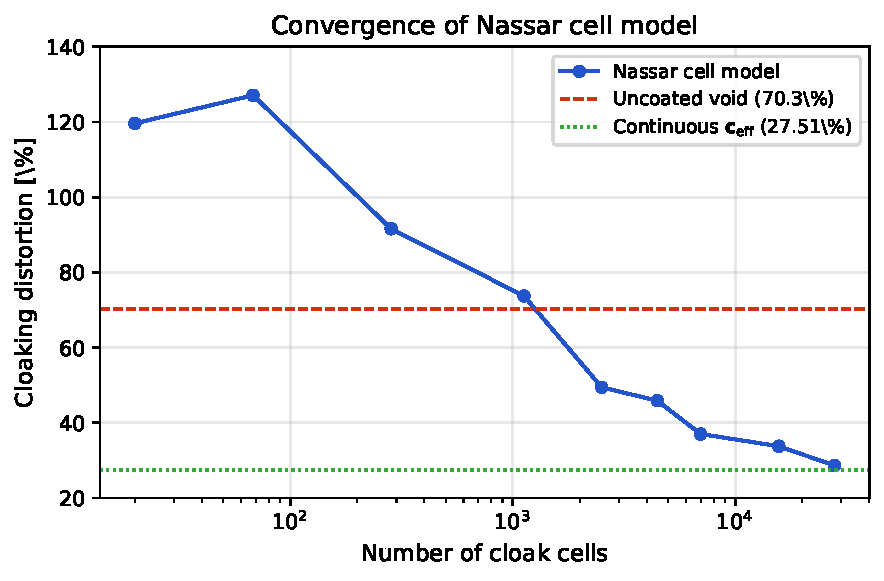
\includegraphics[width=0.75\linewidth]{../figures/nassar_convergence.pdf}
  \caption{Convergence of the Nassar cell model (right-boundary loss).
  As the number of cloak cells increases, the distortion decreases
  from the coarse-grid value
  ($\mathcal{D} \approx 127\%$ at $10\times10$) toward the continuous
  limit ($\mathcal{D} \approx 27.5\%$).
  Above ${\sim}\,60\times60$ cells the cloak outperforms the uncoated
  void (dashed red line), and at $200\times200$ cells the cell model
  approaches the continuous $\mbf{c}_{\mathrm{eff}}$ limit.}
  \label{fig:convergence}
\end{figure}

The convergence is monotonic for grids above $10\times10$
(Table~\ref{tab:convergence}, Fig.~\ref{fig:convergence}):
the cell model begins worse than the bare void at very coarse
resolution ($5\times5$, $10\times10$), because the piecewise-constant
approximation of the singular $\mbf{c}_{\mathrm{eff}}$ near $r_i$
introduces strong impedance mismatches at cell boundaries.
At ${\sim}\,60\times60$ cells the cloaking quality surpasses the
uncoated case, and at $200\times200$ cells the distortion
approaches the continuous limit of~$27.5\%$.

The residual ${\sim}\,28\%$ distortion on the right boundary even
for the continuous cloak is questionable and requires further investigation.

\subsection{Mesh convergence of the continuous $\mbf{c}_{\mathrm{eff}}$ model}

To understand the role of FEM discretisation error,
the continuous $\mbf{c}_{\mathrm{eff}}$ cloak is solved on meshes
ranging from $80\times80$ to $250\times250$ physical elements.

\begin{table}[H]
\centering
\caption{Mesh convergence of the continuous $\mbf{c}_{\mathrm{eff}}$ model.}
\label{tab:ceff_convergence}
\begin{tabular}{@{}lrrr@{}}
\toprule
Mesh & $\mathcal{D}_{\mathrm{right}}$ [\%]
     & $\mathcal{D}_{\mathrm{boundary}}$ [\%]
     & $\mathcal{D}_{\mathrm{outside}}$ [\%] \\
\midrule
$80\times80$   & 41.58 & 4.32 & 4.22 \\
$120\times120$ & 31.70 & 2.49 & 2.35 \\
$160\times160$ & 27.51 & 1.33 & 1.57 \\
$200\times200$ & 27.13 & 1.27 & 1.30 \\
$250\times250$ & 23.02 & 1.04 & 1.06 \\
\bottomrule
\end{tabular}
\end{table}

A power-law fit $\mathcal{D}(h) = \mathcal{D}_\infty + A\,h^p$ to the
right-boundary distortion (where $h = 1/N$ is the characteristic mesh
size) yields convergence exponent $p \approx 1.35$ and asymptote
$\mathcal{D}_\infty \approx 19\%$ (Fig.~\ref{fig:ceff_convergence}).
Extrapolation predicts $\mathcal{D} \approx 21\%$ at $N = 500$ and
$\mathcal{D} \approx 20\%$ at $N = 1000$, indicating that a
significant portion of the $\sim\!28\%$ residual distortion observed
at $160\times160$ is FEM discretisation error rather than an intrinsic
limitation of the continuous cloak.

\begin{figure}[H]
  \centering
  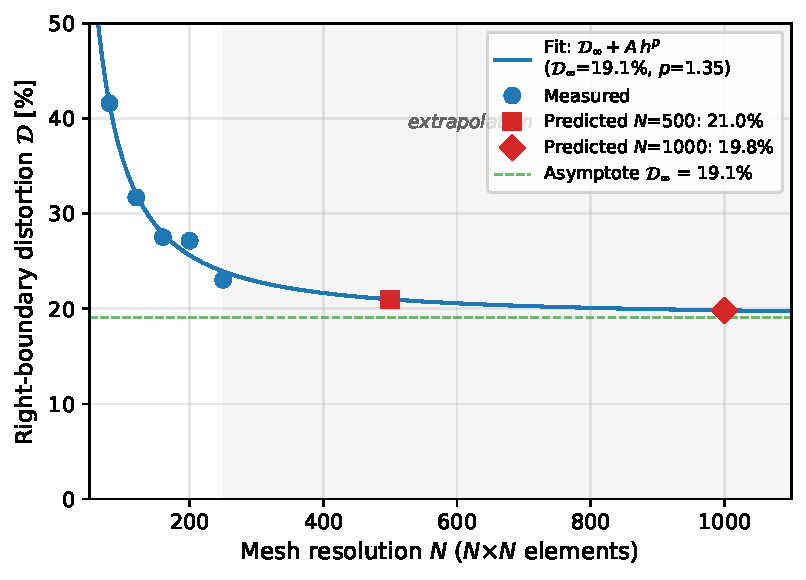
\includegraphics[width=0.75\linewidth]{../figures/continuous_ceff_convergence.pdf}
  \caption{Mesh convergence of the continuous $\mbf{c}_{\mathrm{eff}}$
  model (right-boundary distortion).
  Circles: measured data; solid line: power-law fit
  $\mathcal{D}_\infty + A\,h^{1.35}$ with
  $\mathcal{D}_\infty \approx 19\%$; diamond/square: extrapolated
  predictions.
  The grey region marks the extrapolation range beyond the finest
  computed mesh ($250\times250$).
  Note that the fit has limited data points ($n=5$) and the
  extrapolation carries substantial uncertainty
  ($\mathcal{D}_\infty = 19 \pm 5\%$).}
  \label{fig:ceff_convergence}
\end{figure}

\subsection{Global outside-cloak distortion}

In addition to the right-boundary metric~$\mathcal{D}$, we evaluate
the \emph{outside-cloak distortion} $\mathcal{D}_{\mathrm{out}}$,
defined over all physical-domain nodes outside the cloak annulus:
\be\label{eq:distortion_outside}
  \mathcal{D}_{\mathrm{out}}
  = 100\,\frac{\|\mbf{u}_{\mathrm{cloak}} - \mbf{u}_{\mathrm{ref}}\|_{L^2(\Omega_{\mathrm{phys}} \setminus \overline{\Omega}_{\mathrm{cloak}})}}
              {\|\mbf{u}_{\mathrm{ref}}\|_{L^2(\Omega_{\mathrm{phys}} \setminus \overline{\Omega}_{\mathrm{cloak}})}}\;\;[\%]\,.
\ee
This metric captures the global wavefield perturbation due to the
scatterer, rather than only the shadow-side mismatch.
It is closely related to the objective function used by
Wang et al.~\cite{wang2022} in their data-driven aperiodic
metamaterial cloak design, where the $L^2$ displacement error over
the exterior domain serves as the optimisation target for
inverse-designed cloaks.

Table~\ref{tab:ceff_convergence} shows that
$\mathcal{D}_{\mathrm{out}}$ converges more rapidly than the
right-boundary metric and is already below~$1.1\%$ at $250\times250$.
A power-law fit $\mathcal{D}_{\mathrm{out}}(n) = \mathcal{D}_\infty + A\,n^{-p}$
(where $n$ is the number of outside-cloak nodes) yields
$p \approx 1.37$ and $\mathcal{D}_\infty \approx 0.75\%$
(Fig.~\ref{fig:ceff_outside_convergence}).
Extrapolation predicts $\mathcal{D}_{\mathrm{out}} \approx 0.80\%$ at
$N = 500$ and $\mathcal{D}_{\mathrm{out}} \approx 0.76\%$ at $N = 1000$,
confirming that the continuous $\mbf{c}_{\mathrm{eff}}$ cloak achieves
near-ideal global cloaking (sub-$1\%$ outside distortion) once the mesh
is sufficiently fine.

\begin{figure}[H]
  \centering
  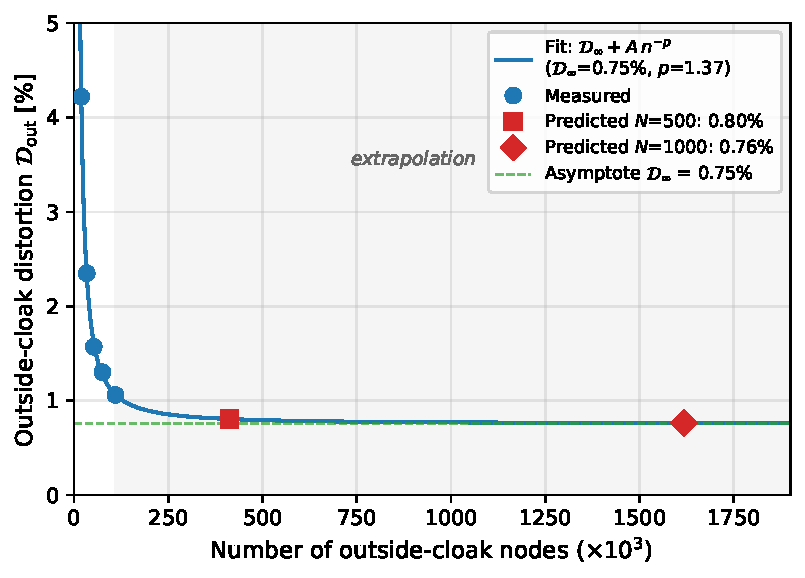
\includegraphics[width=0.75\linewidth]{../figures/continuous_ceff_outside_convergence.pdf}
  \caption{Mesh convergence of the outside-cloak distortion
  $\mathcal{D}_{\mathrm{out}}$ for the continuous
  $\mbf{c}_{\mathrm{eff}}$ model, plotted against the number of
  outside-cloak nodes.
  Circles: measured data; solid line: power-law fit with
  $\mathcal{D}_\infty \approx 0.75\%$ and $p \approx 1.37$;
  diamond/square: extrapolated predictions.
  The asymptotic value $\mathcal{D}_\infty \approx 0.75\%$ serves
  as a reference target for the continuous cloak under this metric,
  comparable to the objective used in~\cite{wang2022}.}
  \label{fig:ceff_outside_convergence}
\end{figure}

\noindent
For comparison, Wang et al.~\cite{wang2022} use the same type of
metric --- relative $L2$ displacement difference over the surrounding
region $\Omega_s$ outside the cloak --- in an elasto-static setting
with a similar circular-void annular-cloak geometry ($r_c = 2\,r_i$).
Their approach differs in two key respects:
(i)~they consider quasi-static loading (compression, pressure, shear)
rather than frequency-domain wave propagation, and
(ii)~they work with classical Cauchy elasticity (orthotropic unit cells
with four independent stiffness parameters $C_{11}, C_{12}, C_{22},
C_{33}$) rather than the Cosserat gauge with broken minor symmetry.
Instead of analytical transformation-elasticity formulas, they employ a
data-driven inverse design that selects aperiodic unit cells from a
precomputed database.
They report:
\begin{quote}
\itshape
``With the designed cloak, the relative difference calculated from
the numerical simulations is reduced from 17.2\% in the voided
structure to 4\% in the cloaked structure, demonstrating a good
cloaking performance.''
\upshape\hfill --- Wang et al.~\cite{wang2022}
\end{quote}
\noindent
Under the analogous global metric $\mathcal{D}_{\mathrm{out}}$,
our continuous $\mbf{c}_{\mathrm{eff}}$ cloak reduces the outside
distortion from $5.18\%$ to an asymptotic ${\sim}\,0.75\%$, substantially below
the $4\%$ achieved by Wang et al., though the comparison is not
strictly apples-to-apples given the different physics.

%% ==================================================================
\section{Gradient-based optimisation of cell parameters}
\label{sec:optimisation}
%% ==================================================================

The entire pipeline --- from cell material parameters through FEM
assembly and solve to the cloaking loss --- is implemented in JAX
and is end-to-end differentiable via implicit adjoint differentiation
through the linear FEM solve.
This enables gradient-based optimisation of the per-cell stiffness
and density to minimise the cloaking distortion directly.

We consider two parameterisation strategies for the material field
over the $80\times80$ cell grid: (i)~direct optimisation of raw
per-cell parameters, and (ii)~neural reparameterisation via a
coordinate-conditioned MLP.

\subsection{Loss function}

The optimisation minimises a composite objective
\be\label{eq:opt_loss}
  \mcl{L}(\mbf{p})
  = \mcl{L}_{\mathrm{cloak}}(\mbf{p})
    + \lambda_{\ell_2}\,\mcl{L}_{\ell_2}(\mbf{p})
    + \lambda_{\mathrm{nb}}\,\mcl{L}_{\mathrm{nb}}(\mbf{p})\,,
\ee
where $\mbf{p} = \{(\mbf{C}^{(k)}_{\mathrm{flat}}, \rho^{(k)})\}_{k=1}^{N_{\mathrm{cells}}}$
collects all per-cell material parameters ($N_{\mathrm{cells}} = 4\,468$ active
cloak cells in the $80\times80$ grid, each with 10 stiffness + 1 density
parameters $\Rightarrow$ ${\sim}\,49\,000$ optimisable DOFs).

The \textbf{cloaking term} measures relative $L^2$ displacement mismatch on
the right physical boundary:
\be
  \mcl{L}_{\mathrm{cloak}}
  = \frac{\|\mbf{u}_{\mathrm{cloak}} - \mbf{u}_{\mathrm{ref}}\|^2}
         {\|\mbf{u}_{\mathrm{ref}}\|^2}\,,
\ee
where $\mbf{u}_{\mathrm{ref}}$ is the reference solution on the full
(void-free) mesh and both solutions share the same mesh nodes on the
measurement boundary (no interpolation needed).

The \textbf{$\ell_2$ regularisation} penalises drift from the initial
(transformation-theory) parameters:
\be
  \mcl{L}_{\ell_2}
  = \frac{\|\mbf{C}_{\mathrm{flat}} - \mbf{C}_{\mathrm{flat}}^{(0)}\|^2}
         {\|\mbf{C}_{\mathrm{flat}}^{(0)}\|^2}
  + \frac{\|\boldsymbol{\rho} - \boldsymbol{\rho}^{(0)}\|^2}
         {\|\boldsymbol{\rho}^{(0)}\|^2}\,,
\ee
where each component is normalised by its own initial norm so that
stiffness and density contribute equally.

The \textbf{neighbour smoothness} term penalises differences between
4-connected adjacent cloak cells:
\be
  \mcl{L}_{\mathrm{nb}}
  = \frac{1}{|\mcl{N}|}\sum_{(i,j)\in\mcl{N}}
    \left(
      \frac{\|\mbf{C}_i - \mbf{C}_j\|^2}{\langle\|\mbf{C}\|^2\rangle}
    + \frac{(\rho_i - \rho_j)^2}{\langle\rho^2\rangle}
    \right),
\ee
where $\mcl{N}$ is the set of neighbour pairs and the denominators are
mean squared magnitudes for scale invariance.

Gradients $\partial\mcl{L}/\partial\mbf{p}$ are computed via JAX-FEM's
\texttt{ad\_wrapper}, which implements implicit adjoint differentiation
through the sparse linear solve.

\subsection{Approach 1: Direct per-cell optimisation}

The most straightforward approach optimises the raw parameter arrays
$\mbf{C}_{\mathrm{flat}}^{(k)} \in \mathbb{R}^{10}$ and
$\rho^{(k)} \in \mathbb{R}$ for each cloak cell directly via
Adam~\cite{kingma2015adam}.
The transformational push-forward~\eqref{eq:Ceff}--\eqref{eq:rhoeff}
evaluated at each cell centre provides the initialisation.

This representation has two drawbacks:
\begin{itemize}
\item \textbf{Memory.}  The number of optimisable parameters scales
  linearly with the number of cells (and cubically with spatial
  resolution if the cell size is reduced to maintain accuracy).
  This is acceptable for small scatterers but does not scale to
  larger structures or 3D.
\item \textbf{Smoothness.}  Raw per-cell parameters do not enforce
  spatial continuity; the material field can develop
  cell-to-cell oscillations that are unphysical and degrade
  convergence.
  This is mitigated by the neighbour regularisation
  $\mcl{L}_{\mathrm{nb}}$ (with weight $\lambda_{\mathrm{nb}}$),
  which acts as a discrete Laplacian penalty on the material field.
\end{itemize}

\noindent
\textbf{Results.}
Starting from the $80\times80$ Nassar cell initialisation
(Table~\ref{tab:convergence}: $\mathcal{D}_{\mathrm{right}} = 45.88\%$),
Adam optimisation with $\mathrm{lr} = 0.025$,
$\lambda_{\ell_2} = 10^{-3}$, $\lambda_{\mathrm{nb}} = 10^{-3}$
over 1\,000 iterations produces:

\begin{table}[H]
\centering
\caption{Cloaking distortion: analytical initialisation vs.\ optimised
$80\times80$ cells vs.\ continuous $\mbf{c}_{\mathrm{eff}}$.}
\label{tab:opt_results}
\begin{tabular}{@{}lrrr@{}}
\toprule
Configuration
  & $\mathcal{D}_{\mathrm{right}}$ [\%]
  & $\mathcal{D}_{\mathrm{boundary}}$ [\%]
  & $\mathcal{D}_{\mathrm{outside}}$ [\%] \\
\midrule
Uncoated void           & 70.31 & --- & 5.18 \\
Nassar $80\times80$ (init) & 45.88 & --- & --- \\
Continuous $\mbf{c}_{\mathrm{eff}}$ & 27.51 & 1.33 & 1.57 \\
\midrule
Optimised $80\times80$ (direct) & \textbf{0.09} & \textbf{1.58} & \textbf{1.74} \\
\bottomrule
\end{tabular}
\end{table}

The right-boundary distortion drops from $45.88\%$ to $0.09\%$
--- essentially perfect cloaking on the shadow side --- which is
substantially better than the continuous $\mbf{c}_{\mathrm{eff}}$ model
($27.51\%$).
The boundary and outside-cloak metrics ($1.58\%$ and $1.74\%$,
respectively) are comparable to the continuous model at the same
$160\times160$ FEM mesh resolution (Table~\ref{tab:ceff_convergence}).
This indicates that the optimiser exploits the additional degrees of
freedom (broken minor symmetry, non-analytical density profile) to
compensate for both the piecewise-constant discretisation error and
the intrinsic limitations of the radial blow-up transformation.

\subsection{Approach 2: Neural reparameterisation}
\label{sec:neural_reparam}

Instead of optimising raw per-cell arrays, we reparameterise the material
field through a small coordinate-conditioned MLP:
\be
  \Phi_\theta \colon (x, y) \;\mapsto\;
  (\mbf{C}_{\mathrm{flat}},\, \rho)\,,
\ee
where $\theta$ denotes the network weights.
The MLP is evaluated at each cell centre to produce the material
parameters, which are then expanded to FEM quadrature points exactly
as in the direct approach.
Optimisation proceeds over $\theta$ rather than the cell arrays;
gradients flow through the FEM adjoint and then through the network
via standard backpropagation.

This is conceptually analogous to the neural implicit representations
used in computer graphics (NeRF~\cite{mildenhall2020nerf} and
related work) but applied to physical material fields rather than
radiance.
The key advantages are:
\begin{itemize}
\item \textbf{Implicit smoothness.}  Neural networks are smooth
  functions of their inputs by construction, so the material field
  is spatially continuous without explicit neighbour regularisation
  ($\lambda_{\mathrm{nb}} = 0$).
\item \textbf{Compact representation.}  A 4-layer MLP with 256 hidden
  units has ${\sim}\,200\text{k}$ weights, which parameterises the
  ${\sim}\,49\text{k}$ cell values through a lower-dimensional manifold
  that encodes spatial correlations.
\item \textbf{Resolution-independent.}  The same network can be
  evaluated at arbitrary cell centres, enabling coarse-to-fine
  transfer without retraining.
\end{itemize}

Following Sitzmann et al.~\cite{sitzmann2020siren}, we use Fourier
input features (sinusoidal positional encoding of the normalised cell
coordinates) to allow the network to represent high-frequency spatial
variations.
SIREN-style periodic activations ($\sin$ instead of $\tanh$) are a
natural alternative that may further improve the representation of
sharp material transitions near the cloak boundaries; this is left
for future experiments.

\paragraph{Transformation prior.}
Crucially, the network does \emph{not} learn the full material field
from scratch.  Instead, it learns a \textbf{residual correction} to the
analytical transformation-elasticity solution.
The last network layer is initialised near zero
($\mbf{W} \leftarrow 0.01\,\mbf{W}$, $\mbf{b} \leftarrow \mbf{0}$),
so at step~0 the material field recovers the analytical initialisation
exactly. Two scaling strategies for the residual are natural:

\medskip\noindent
\paragraph{Additive (absolute) residual.}
\be\label{eq:neural_additive}
  \mbf{C}_{\mathrm{flat}}(x,y)
  = \mbf{C}_{\mathrm{flat}}^{(0)}(x,y)
    + \epsilon\,\boldsymbol{\sigma}_C \odot \Phi_\theta^{(C)}(x,y)\,,
\ee
where $\boldsymbol{\sigma}_C$ is the per-component standard deviation
of the initial field across cloak cells and $\epsilon$ is a global
output scale.
This is simple but problematic: the effective stiffness
$\mbf{c}_{\mathrm{eff}}$ varies by orders of magnitude across the
cloak (near-zero radial stiffness at $r \to r_i$, background-level
at $r \to r_c$), so a single additive scale produces relative
perturbations that are either too small where $C$ is large or too
large where $C$ is small.

\medskip\noindent
\paragraph{Multiplicative (relative) residual.}
\be\label{eq:neural_relative}
  \mbf{C}_{\mathrm{flat}}(x,y)
  = \mbf{C}_{\mathrm{flat}}^{(0)}(x,y)
    \odot \bigl(1 + \epsilon\,\Phi_\theta^{(C)}(x,y)\bigr)\,,
  \qquad
  \rho(x,y)
  = \rho^{(0)}(x,y)
    \,\bigl(1 + \epsilon\,\Phi_\theta^{(\rho)}(x,y)\bigr)\,,
\ee
where $\epsilon$ is the output scale (default 0.1).
Each cell's correction is proportional to its own initial value,
so the relative perturbation is spatially uniform regardless of the
local magnitude of $\mbf{c}_{\mathrm{eff}}$.
This eliminates the need for per-component normalisation and produces
well-conditioned gradients across the entire cloak.
We use this form in practice.

\noindent
\paragraph{Preliminary results.}
Neural reparameterisation has been implemented and produces
valid gradients through the full pipeline.
Systematic comparison with the direct approach (convergence speed,
final loss, generalisation across frequencies) is ongoing.
Additional regularisation strategies for material physical plausibility
(e.g.\ positive-definite stiffness) are also being explored.

\begin{figure}[H]
  \centering
  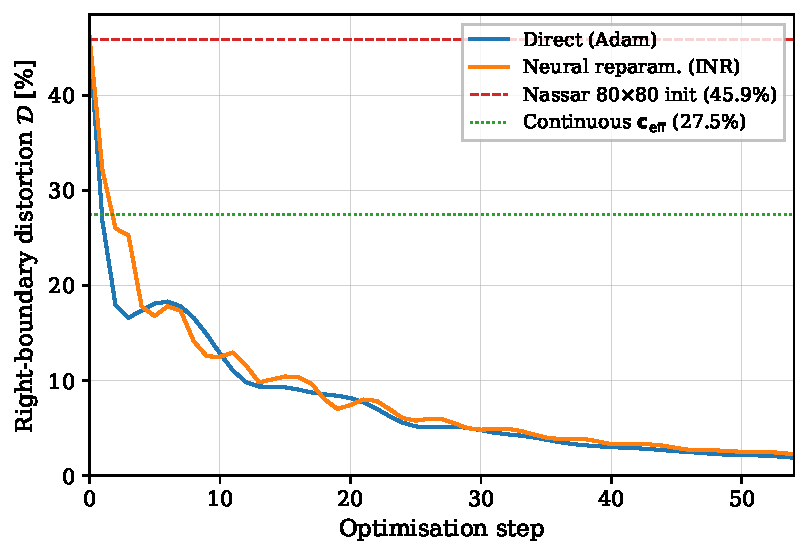
\includegraphics[width=0.75\linewidth]{../figures/convergence_comparison.pdf}
  \caption{Convergence of right-boundary distortion $\mathcal{D}$ during
  optimisation for the direct (Adam) and neural reparameterisation (INR)
  approaches on the $80\times80$ grid.
  Both methods drop below the continuous $\mbf{c}_{\mathrm{eff}}$ baseline
  ($27.5\%$) within ${\sim}\,10$ steps and reach ${\sim}\,3\%$ by step~50.
  Dashed/dotted lines mark the Nassar $80\times80$ initialisation and the
  continuous transformation-elasticity limit.}
  \label{fig:convergence_comparison}
\end{figure}

\printbibliography

\end{document}
